\section{Приложение}
\subsection{Приложение 1} \label{Приложение 1}
Рассмотрим обычную схему откачки. Разделим вакуумную систему на две части: «откачиваемый объем» (в состав которого включим используемые для работы части установки) и «насос», к которому, кроме самого насоса, отнесём трубопроводы и краны, через которые производится откачка нашего объема. Пусть $Q_\text{д}$ - количество газа, десорбирующего с поверхности откачиваемого объема в единицу времени, $Q_\text{и}$ - количество газа, проникающего в единицу времени в этот объем извне - через течи, $Q_\text{н}$ - количество газа, поступающего в систему из насоса в единицу времени. Будем измерять количество газа $Q_\text{д}, Q_\text{и}, Q_\text{н}$ в единицах $PV$ с точностью до константы $\frac{RT}{\mu}$. Выражение, описывающее процесс откачки, имеет вид
\begin{equation}
    -VdP = (PW - Q_\text{д} - Q_\text{и} - Q_\text{н})dt \label{eq: 1}
\end{equation}
Левая часть равна убыли массы газа в откачиваемом объеме, правая определяет количество газа, уносимое насосом, и количество прибывающего вследствие указанных выше причин за время $dt$.

При достижении предельного вакуума $P_\text{пр}$ 
\begin{equation}
    \frac{dP}{dt} = 0 \label{eq: 2}
\end{equation}
Из \eqref{eq: 1} с учетом \eqref{eq: 2} следует
\begin{equation}
    P_\text{пр} W = Q_\text{д} + Q_\text{и} + Q_\text{н} \label{eq: 3}
\end{equation}
Интегрируя выражение \eqref{eq: 1} и, используя \eqref{eq: 3}, получаем 
\begin{equation}
    P - P_\text{пр} = (P_0 - P_\text{пр})\exp({-\frac{W}{V}}) \label{eq: 4}
\end{equation}
где $P_0$ - начальное давление в системе. Обычно оно велико по сравнению с $P_\text{пр}$, следовательно \eqref{eq: 4} можно записать так
\begin{equation}
    P = P_\text{пр} + P_0\exp({-\frac{W}{V}}) \label{eq: 5}
\end{equation}

Рассмотрим, чем определяется скорость откачки откачивающей системы. Откачивающая система состоит из насоса и трубопроводов, соединяющих насос с откачиваемым объемом. При математическом описании откачивающей системы возникают уравнения, очень похожие на уравнения Кирхгофа, описывающие
протекание тока в электрических цепях. Перепад давления $\Delta P$ заменяет разность электрических потенциалов, поток газа — силу тока,
а пропускная способность $C$ элементов вакуумной системы — проводимость элементов цепи. Закон сложения пропускных способностей аналогичен закону сложения проводимостей. При последовательном соединении элементов
\begin{equation}
    \frac{1}{W} = \frac{1}{W_\text{н}} + \frac{1}{C_1} + \frac{1}{C_2} + \dots \label{eq: kirh}
\end{equation}
где $W_\text{н}$ - проводимость насоса, $C_1, C_2$ - проводимости трубопровода, 
$W$ - проводимость откачивающей системы.

\newpage
\subsection{Приложение 2} \label{Приложение 2}
\textbf{Вывод выражения для скорости откачки при наличии в системе искусственной течи}

Рассмотрим высоковакуумную часть установки при отсутствии искусственной течи, то есть закрытом кране $K_6$. В выделенный объем в единицу времени будет натекать масса $Q_1$ воздуха, но в то же время насос будет откачивать за единицу времени массу газа $P_\text{пр}W$, где $P_\text{пр}$ - предельное давление в системе в стационарном состоянии. Из этого следует, что справедливо
\begin{equation}
    P_\text{пр}W = Q_1 \label{eq: sist1}
\end{equation}

Рассмотрим систему с искусственной течью через капилляр $K_6-K_5$. Измерим новое предельное установившееся давление $P_\text{уст}$ в высоковакуумной части и давление на втором конце капилляра на входе в форвакуумный насос. С помощью выражения \eqref{eq: C} определён массовый расход $\frac{d(PV)}{dt}$ воздуха через капилляр. Справедливо выражение, аналогичное \eqref{eq: sist1} с добавлением массового расхода через капилляр
\begin{equation}
    P_\text{уст}W_\text{теч} = Q_1  + \frac{d(PV)}{dt} \label{eq: sist2}
\end{equation}

Из \eqref{eq: sist1} и \eqref{eq: sist2} следует, что 
\begin{equation}
    W_\text{теч} = \frac{\frac{d(PV)_\text{кап}}{dt}}{P_\text{уст} - P_\text{пр}}
\end{equation}
\newpage
\subsection{Приложение 3} \label{Приложение 3}
Схема экспериментальной установки приведена на рисунке 1.
\begin{figure}[ht]
    \label{figure1}
    \center{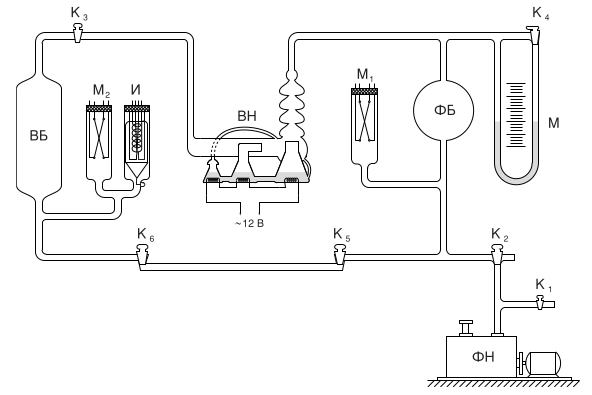
\includegraphics[scale=0.4]{img/exp_ust.png}}
    \caption{Экспериментальная установка для измерения скорости откачки воздуха}
\end{figure}

Установка изготовлена из стекла и состоит из форвакуумного баллона (ФБ), высоковакуумного диффузионного насоса (ВН), высоковакуумного баллона (ВБ), масляного (М) и ионизационного (И) манометров, термопарных манометров
($M_1, M_2$), форвакуумного насоса (ФН) и соединительных кранов $K_1,
K_2,\dots,K_6$.

Кран $К_1$ используется для заполнения форвакуумного насоса и вакуумной установки атмосферным воздухом. Трехходовой кран $К_2$ служит для соединения форвакуумного насоса с установкой или атмосферой. Кран $К_3$ отделяет высоковакуумную часть установки от форвакуумной. Кран $К_4$ соединяет между собой колена масляного манометра. Он должен быть открыт во всё время работы установки и закрывается лишь при измерении давления в форвакуумной части. Краны $К_5$ и $К_6$ стоят по концам капилляра и соединяют его с форвакуумной и
высоковакуумной частями установки.

\subsubsection{Форвакуумный насос (ФН)}
Устройство и принцип действия схематически показаны на рисунке 2.
\begin{figure}[ht]
    \label{figure2}
    \center{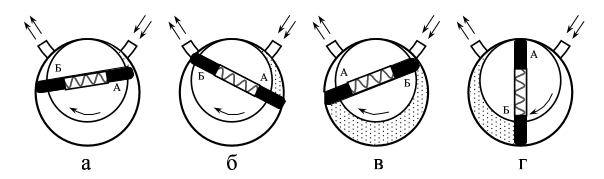
\includegraphics[scale=0.4]{img/fn.png}}
    \caption{Принцип работы форвакуумного насоса. В положениях "а", "б" пластина "А" засасывает разреженный воздух из откачиваемого объёма, а пластина "Б" вытесняет ранее захваченный воздух в атмосферу, в положениях "в" и "г" пластины поменялись ролями.}
\end{figure}

В цилиндрической полости массивного корпуса размещён эксцентрично ротор так, что он постоянно соприкасается своей верхней частью с корпусом. В диаметральный разрез ротора вставлены две пластины, раздвигаемые пружиной и плотно прижимаемые к поверхности полости. Они разделяют объём между ротором и корпусом на две части.

Действие насоса ясно из изображенных на рис. 2 последовательных положений пластин при вращении ротора по часовой стрелке.
В положении «а» газ из откачиваемого объема поступает в пространство между пластиной «А» и линией соприкосновения корпуса и ротора. По мере вращения это пространство увеличивается (рис. 2 б), пока вход в него не перекроет другая пластина «Б» (рис. 2 в). После того как пластина «А» пройдет выходное отверстие и линию соприкосновения (рис. 2 г), лопасть «Б» будет сжимать следующую порцию газа и вытеснять его через клапан в атмосферу.

\subsubsection{Диффузионный насос (ВН)}
Схема устройства диффузионного насоса представлена на рисунке 3.
\begin{figure}[ht]
    \label{figure3}
    \center{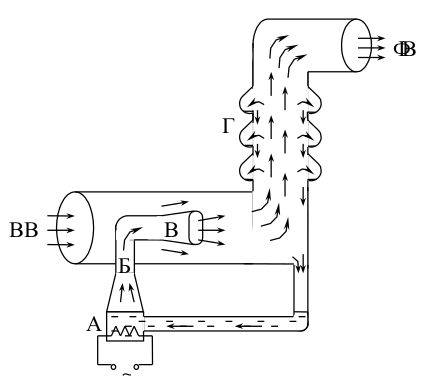
\includegraphics[scale=0.4]{img/dn.png}}
    \caption{Устройство диффузионного насоса}
\end{figure}

Откачивающее действие диффузионного насоса основано на диффузии молекул разреженного воздуха в струю паров масла. Попавшие в струю молекулы газа увлекаются ею и уже не возвращаются назад. На прежнем их месте образуется пустота, которая немедленно заполняется следующими порциями газа, увеличивая степень разрежения газа в окрестности струи и оказывая таким образом сильное откачивающее воздействие на весь газ в откачиваемом объеме.

Масло, налитое в сосуд А, подогревается электрической печкой. Пары масла поднимаются по трубе Б и вырываются из сопла В. Струя паров увлекает молекулы газа, которые поступают из откачиваемого сосуда через трубку ВВ. Дальше смесь попадает в вертикальную трубу Г. Здесь масло осаждается на стенках трубы и маслосборников и стекает вниз, а оставшийся газ через трубу ФВ откачивается форвакуумным насосом.

Диффузионный насос, используемый в установке, имеет две ступени, и соответственно, два сопла. Одно сопло вертикальное (первая ступень), второе сопло горизонтальное (вторая ступень). За второй ступенью имеется еще одна печь, но пар из этой печи поступает не в сопло, а по тонкой трубке подводится ближе к печке первой ступени. Эта печь осуществляет фракционирование
масла. Легколетучие фракции масла, испаряясь, поступают в первую ступень, обогащая ее легколетучей фракцией масла. По этой причине
плотность струи первой ступени выше, и эта ступень начинает откачивать при более высоком давлении в форвакуумной части установки. Вторая ступень обогащается малолетучими фракциями. Плотность струи второй ступени меньше, но меньше и давление насыщенных паров масла в этой ступени. Соответственно, в откачиваемый объем поступает меньше паров масла, и его удается откачать до более высокого вакуума, чем если бы мы работали только с одной ступенью.

Спираль, опущенная в масло, подогревается переменным током ($U \approx 12\text{В}$). Ток регулируется автотрансформатором в пределах от $1 до 1,5\text{А}$. При включении подогрева давление в системе сначала возрастает вследствие выделения растворенного в масле воздуха. Минут через 10 после начала подогрева начинается интенсивное испарение масла, заметное по появлению на стенках насоса пленки конденсирующихся паров.

\subsubsection{Термопарный манометр ($M_1, M_2$)}
Схема устройства термопарного манометра приведена на рисунке 4.
\begin{figure}[ht]
    \label{figure4}
    \center{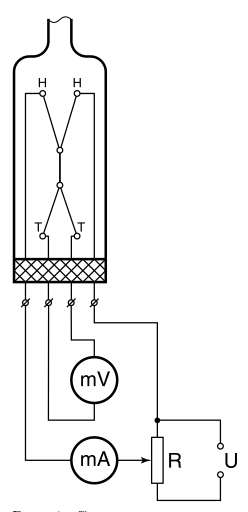
\includegraphics[scale=0.4]{img/tm.png}}
    \caption{Устройство термопарного манометра}
\end{figure}

Чувствительным элементом манометра является платино-платинородиевая термопара, спаянная с никелевой нитью накала и заключённая в стеклянный баллон (лампа ЛТ-2 или ПМТ-2).По нити накала НН пропускается ток постоянной величины. Для установки тока служит потенциометр R, расположенный на передней панели вакуумметра. Термопара ТТ присоединяется к милливольтметру, показания которого определяются температурой нити накала и зависят от отдачи тепла в окружающее пространство. Градуировочная кривая термопары ПМТ-2 приведена на рисунке 5.
\begin{figure}[ht]
    \label{figure5}
    \center{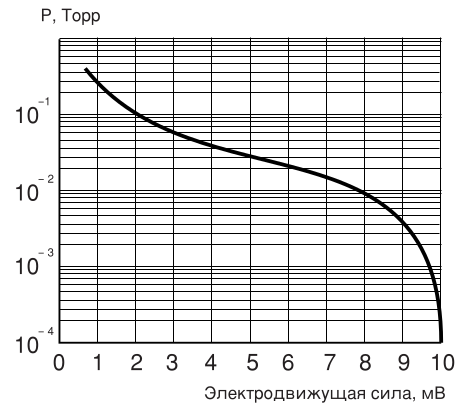
\includegraphics[scale=0.4]{img/gr_kr.png}}
    \caption{Градуировочная кривая термопары ПМТ-2}
\end{figure}

\subsubsection{Ионизационный манометр (И)}
Схема ионизационного манометра приведена на рисунке 6.
\begin{figure}[ht]
    \label{figure6}
    \center{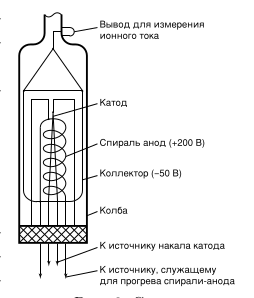
\includegraphics[scale=0.4]{img/im.png}}
    \caption{Схема ионизационного манометра}
\end{figure}

Он представляет собой трехэлектродную лампу. Электроны испускаются накаленным катодом и увлекаются электрическим полем к аноду, имеющему вид редкой спирали. Проскакивая за ее витки, электроны замедляются полем коллектора и возвращаются к катоду, а от него вновь увлекаются к аноду. Прежде чем осесть на аноде, они успевают много раз пересечь пространство между катодом и коллектором. На своем пути электроны ионизуют молекулы газа. Ионы, образовавшиеся между анодом и коллектором, притягиваются полем коллектора и определяют его
ток. Ионный ток в цепи коллектора пропорционален плотности газа и поэтому может служить мерой давления.
\newpage
\subsection{Приложение 4} \label{Приложение 4}
\textbf{Способ измерения объемов форвакуумной и высоковакуумной частей установки}

Необходимо открыть все краны, кроме $K_1, K_2$ и впустить через них атмосферный воздух в систему. Затем закрываем краны $K_5, K_6$ и таким образом запираем воздух при атмосферном давлении $P_\text{атм} = (748 \pm 1)\text{торр}$ в капилляре объемом $V_\text{кап}= 50\text{см}^3$. Подключаем установку к форвакуумному насосу, открыв краны $K_1, K_2$, и откачиваем систему до давления $10^{-2} \text{торр}$. После достижения необходимого давления отсоединяем установку от насоса и краном $K_3$ отделяем высоковакуумную и форвакуумную части установки. Откроем кран $K_4$, чтобы привести в готовность к измерениям масляный манометр. Откроем кран $K_5$, воздух распространится из капилляра в форвакуумную часть установки, измерим давление $P_1 = 18.6\text{торр}$ по масляному манометру. С помощью закона Бойля-Мариотта определим объем $V_\text{фв} = 11.8\text{торр}$ форвакуумной части установки \eqref{eq: Vfv}.
\begin{equation}
    P_{\text{атм}}V_\text{кап} = P_1 (V_\text{кап}+V_\text{фв}) \rightarrow V_\text{фв} = \frac{P_{\text{атм}}V_\text{кап}}{P_1} - V_\text{кап} \label{eq: Vfv}
\end{equation}

Откроем кран $K_3$, газ распространится на всю установку. Снова измерим давление $P_2$ в системе с помощью масляного манометра. Из закона Бойля-Мариотта определим объем $V_\text{вв}$ высоковакуумной части установки \eqref{eq: Vvv}.
\begin{equation}
    P_{\text{атм}}V_\text{кап} = P_2 (V_\text{кап}+V_\text{фв}+V_\text{вв}) \rightarrow V_\text{вв} = \frac{P_{\text{атм}}V_\text{кап}}{P_2} - V_\text{кап} - V_\text{фв} \label{eq: Vvv}
\end{equation}
\newpage
\subsection{Приложение 5} \label{Приложение 5}
\begin{table}[h]
    \centering
    \begin{tabular}{|c|c|}
    \hline
    $t, \text{мс}$ & $P\cdot 10^{-4}, \text{мм. рт. ст.}$ \\ \hline
    48 & 5.4 \\ \hline
    51 & 4.4 \\ \hline
    54 & 2.7 \\ \hline
    57 & 1.7 \\ \hline
    60 & 1.2 \\ \hline
    63 & 0.95 \\ \hline 
    66 & 0.83 \\ \hline
    69 & 0.77 \\ \hline
    72 & 0.74 \\ \hline
    75 & 0.73 \\ \hline
    78 & 0.72 \\ \hline
    81 & 0.71 \\ \hline
    84 & 0.70 \\ \hline
     
\end{tabular}
    \caption{Зависимость давления $P$ воздуха от времени $t$ при улучшении вакуума}
    \label{tab:t1}
\end{table}
\newpage
\subsection{Приложение 6} \label{Приложение 6}
\begin{table}[ht]
    \centering
    \begin{tabular}{|c|c|}
    \hline
    $t, \text{мс}$ & $P\cdot 10^{-4}, \text{мм. рт. ст.}$ \\ \hline
    0  & 0.69 \\ \hline
    3  & 0.83 \\ \hline
    6  & 1.1 \\ \hline
    9  & 1.5 \\ \hline
    12 & 1.8 \\ \hline
    15 & 2.1 \\ \hline
    18 & 2.4 \\ \hline
    21 & 2.7 \\ \hline
    24 & 3.0 \\ \hline
    27 & 3.3 \\ \hline
    30 & 3.6 \\ \hline
    33 & 3.9 \\ \hline
    36 & 4.3 \\ \hline
    39 & 4.6 \\ \hline
    42 & 4.9 \\ \hline
    45 & 5.1 \\ \hline
    48 & 5.4 \\ \hline
     
\end{tabular}
    \caption{Зависимость давления $P$ воздуха от времени $t$ при ухудшении вакуума}
    \label{tab:t1}
\end{table}
